% 第 21 题【A】外接圆图：按固定源 400 dpi 位图实测值复刻（1 bp → 0.03515 cm）。
% 原点取圆心（源页 (710.7, 183.2)），y 向上。
% 圆半径 56.6（笔迹中线）；弦 AB/AC/BC/AE/BE 全为实线、两端均止于圆上（无圆外延长段）；
% 圆为按题设 AB=AC 精确作图（B、C 关于过圆心竖轴镜像，互差 0.12 pt）；圆心实心点 U+2022（直径 2.52，落于圆心）。全图无虚线、无箭头、无直角记号。
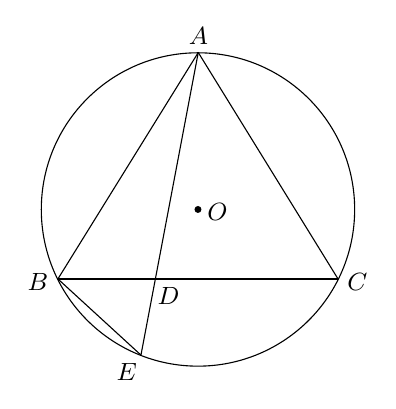
\begin{tikzpicture}[line cap=round,line join=round,font=\small,x=0.03515cm,y=0.03515cm]
\draw (0,0) circle (56.6);   % 外接圆 ⊙O
\draw (0.1,56.7)--(-50.6,-25.1);   % 弦 AB
\draw (0.1,56.7)--(50.6,-25.1);   % 弦 AC
\draw (-50.6,-25.1)--(50.6,-25.1);   % 弦 BC
\draw (0.1,56.7)--(-20.6,-52.6);   % 弦 AE
\draw (-50.6,-25.1)--(-20.6,-52.6);   % 弦 BE
\fill (0,0) circle (1.26pt);   % 圆心实心点（照源字形 U+2022，直径 2.52）
% ===== 标注（照源字框中心，显式坐标）=====
\node[anchor=center,inner sep=0] at (0.2,62.6) {\(A\)};
\node[anchor=center,inner sep=0] at (-57.8,-26.3) {\(B\)};
\node[anchor=center,inner sep=0] at (57.6,-26.3) {\(C\)};
\node[anchor=center,inner sep=0] at (-10.6,-31.2) {\(D\)};
\node[anchor=center,inner sep=0] at (-25.7,-58.7) {\(E\)};
\node[anchor=center,inner sep=0] at (7,-1) {\(O\)};
\end{tikzpicture}
